\documentclass[11pt,a4paper]{article}
\usepackage[T1]{fontenc}
\usepackage[utf8]{inputenc}
\usepackage{lmodern,microtype}
\usepackage[margin=25mm,headheight=14pt]{geometry}
\usepackage{graphicx,booktabs,array,longtable,amsmath}
\usepackage[round,authoryear]{natbib}
\usepackage{xcolor}
\usepackage[hidelinks]{hyperref}
\usepackage{fancyhdr}
\usepackage{enumitem}
\usepackage{placeins}
\definecolor{ink}{HTML}{163746}
\hypersetup{pdftitle={Comparative Deep Learning for Testicular Ultrasound Classification},pdfauthor={David Ongaro Mauti Ethan},pdfsubject={DSA 8401 MSc Capstone Report}}
\pagestyle{fancy}
\fancyhf{}
\fancyhead[L]{\small Testicular ultrasound classification}
\fancyhead[R]{\small DSA 8401}
\fancyfoot[C]{\thepage}
\setlength{\parindent}{0pt}
\setlength{\parskip}{6pt}
\setlength{\emergencystretch}{2em}
\renewcommand{\arraystretch}{1.16}
\setlist{nosep,leftmargin=*}
\newcommand{\code}[1]{\texttt{\detokenize{#1}}}
\newcommand{\source}[1]{{\footnotesize\textit{Evidence:} #1}}
\newcommand{\mobile}{MobileNetV3-Small}
\begin{document}
\begin{titlepage}
\centering
{\Large Strathmore University\par}
\vspace{4mm}
{\large iLabAfrica\par}
{\large MSc in Data Science and Analytics\par}
\vspace{20mm}
{\color{ink}\LARGE\bfseries Comparative Deep Learning for Testicular Ultrasound Classification\par}
\vspace{6mm}
{\Large Predictive Performance, Explainability, and Computational Efficiency\par}
\vspace{20mm}
{\large David Ongaro Mauti Ethan\par}
\vspace{3mm}
{\large Registration number: 191204\par}
\vspace{15mm}
{\large DSA 8401 --- Applied Machine Learning\par}
{\large Capstone Project Report\par}
\vfill
{Prepared: 18 November 2026\par}
{Revised: 19 November 2026\par}
{Submission deadline: 20 November 2026\par}
\vspace{10mm}
\begin{minipage}{0.84\textwidth}
\small This study evaluates image-level research classifiers. Verified patient and centre identifiers were unavailable. The results do not establish patient-independent or centre-held-out performance, clinical validation, or suitability for diagnosis.
\end{minipage}
\end{titlepage}
\pagenumbering{roman}
\section*{Abstract}
\addcontentsline{toc}{section}{Abstract}
% ABSTRACT_BEGIN
Automated classification of testicular ultrasound images requires evaluation that accounts for limited data, class imbalance and deployment constraints. This study compares a Custom CNN trained from scratch with an ImageNet-initialized ResNet18, followed by a post-hoc exploratory MobileNetV3-Small with frozen features. The local TesticulUS classification subset contains 860 grayscale images: 696 homogeneous and 164 inhomogeneous. A fixed stratified image-level split allocated 602 images to training and 129 each to validation and testing. Class-weighted training and validation-loss checkpoint selection were followed by validation-only positive-class F1 threshold selection. Saved predictions and experimental records were audited without repeating test inference. On the common test partition, ResNet18 achieved the highest ROC-AUC (0.7473), Average Precision (0.5220) and sensitivity (0.6400). MobileNetV3-Small achieved accuracy 0.8217 and F1 0.4390, but sensitivity was 0.3600; the majority-class accuracy baseline was 0.8062. Median model-forward latency on an Intel Core i7-7500U CPU was 10.59 ms for MobileNet, compared with 62.17 ms for ResNet18. Grad-CAM, threshold-aware FastAPI inference and Docker deployment were implemented and technically verified. These checks do not establish anatomical explanation quality. Missing patient and centre mappings, 25 positive test images, single-seed experiments and MobileNet's post-hoc addition limit generalization and comparative inference. The evidence supports a reproducible research application and a measured performance--efficiency trade-off, while patient-independent external evaluation remains necessary before any clinical interpretation.
% ABSTRACT_END

\vspace{3mm}
\textbf{Keywords:} testicular ultrasound; transfer learning; class imbalance; decision thresholds; Grad-CAM; CPU inference.
\newpage
{\small\setlength{\parskip}{0pt}\tableofcontents}
\newpage
\pagenumbering{arabic}

\section{Introduction}
\subsection{Problem and motivation}
Testicular ultrasound provides images of tissue appearance that can support assessment of testicular structure. Parenchymal inhomogeneity is the image characteristic considered in the TesticulUS classification work \citep{2025ICIAP}. This project addresses a narrower computational task: predicting the supplied homogeneous or inhomogeneous image label. It does not predict infertility, malignancy, treatment need or a patient diagnosis. This distinction matters because an image-level appearance label is neither a clinical outcome nor a complete examination.

A useful classification experiment must contend with the data actually available. In the local labelled subset, homogeneous images outnumber inhomogeneous images by approximately 4.24 to one. A system can therefore achieve high accuracy while failing to identify any positive image. The small sample also limits how confidently differences between models can be interpreted. Consequently, this study examines ranking discrimination, positive-class performance and computational cost together, rather than treating accuracy as a sufficient endpoint.

Transfer learning offers an established way to initialize a classifier when labelled examples are limited, but its value depends on the target task \citep{raghu2019}. A scratch-trained CNN provides a compact reference, while ResNet18 introduces a deeper, pretrained representation. A later exploratory \mobile{} experiment addresses a different practical question: whether a frozen lightweight representation can offer a useful CPU inference trade-off. This sequence also creates an interpretive constraint: the third architecture was added after the first two test results were known.

\subsection{Research questions and objectives}
The central question is how these completed modelling configurations trade image-level discrimination and positive-class detection against inference cost on the available dataset. Four questions organize the study:
\begin{enumerate}
\item How do the scratch-trained Custom CNN and ImageNet-initialized ResNet18 differ on the same fixed test images?
\item How does validation-based F1 threshold selection affect the observed precision, sensitivity and specificity?
\item What exploratory performance--efficiency trade-off is observed for a frozen-feature \mobile{} classifier?
\item Can the frozen models, preprocessing and thresholds be restored consistently through explainability tooling and a containerized prediction service?
\end{enumerate}
The objectives are therefore to construct an auditable classification pipeline, compare saved model outcomes with imbalance-aware metrics, separate weight selection from decision-threshold selection, assess measured CPU efficiency, and verify reproducible inference interfaces. Grad-CAM is included as an inspection capability; the available evidence does not support a separate scientific claim about explanation quality.

\subsection{Scope and contribution}
The initial project framing considered cross-centre distribution shift. Although the provider describes a multicentre collection, verified patient/examination identifiers and per-image centre assignments were unavailable in the local copy. A genuine centre-held-out design could not be implemented. The completed study consequently uses a provisional stratified image-level evaluation. Scanner appearance and filenames were not used to invent group assignments.

The contribution is an evidence-linked comparison and working research application, rather than a new network architecture. It combines explicit split manifests, training-label class weighting, validation-selected thresholds, preserved predictions and hashes, model-specific preprocessing, Grad-CAM, and API/Docker verification. The report interprets the resulting evidence and its limits; operational installation instructions remain in the repository README.

\section{Related work and technique justification}
\subsection{TesticulUS classification and segmentation studies}
In their ICIAP 2025 paper, \citet{2025ICIAP} study testicular inhomogeneity classification using ResNet-based supervised and unsupervised pretraining, including diffusion-generated ultrasound data. Their findings motivate investigating initialization when target labels are scarce. The present study does not reproduce their synthetic-data pipeline or evaluation design, and its metrics should not be read as a direct replication or a leaderboard comparison. In particular, synthetic pretraining and its additional data were not used here.

\citet{2026BMVC} introduce the real multicentre TesticulUS release and Cond-UNet, an organ-conditioned segmentation architecture. This provides important dataset context and illustrates an efficiency-oriented approach to ultrasound analysis. However, Cond-UNet predicts segmentation masks; it is not one of this project's classification models. The available masks could support a future region-of-interest experiment, but introducing segmentation would change the present input definition and require a separately designed comparison. The official resources distinguish the earlier synthetic release from the later real-image release \citep{dataset}.

Together, these studies establish the relevance of testicular ultrasound learning while also showing why task and protocol matching matter. Segmentation quality cannot substitute for inhomogeneity classification performance. Similarly, the fact that images originated from two institutions cannot establish cross-centre performance when their local image-level affiliations are unknown.

\subsection{Scratch training, transfer learning and efficient architectures}
A CNN learns local spatial filters and composes them into image-level features. The Custom CNN tests whether a small, directly adapted grayscale network can learn a useful representation without external initialization. Its limited parameter count and global pooling constrain the classifier size, but neither guarantees adequate generalization from 602 training images.

Residual learning uses shortcut connections to make deeper representations easier to optimize \citep{he2016}. ResNet18 was selected as a manageable pretrained comparator rather than a large architecture search. Its full feature hierarchy was trainable, allowing adaptation to ultrasound. This configuration addresses a practical modelling choice, but it changes both architecture and initialization relative to the Custom CNN. Thus, an observed advantage cannot be attributed solely to pretraining or solely to residual connections.

\citet{raghu2019} demonstrate that natural-image transfer benefits are task-dependent in medical imaging and that lightweight models can sometimes be competitive. Their analysis cautions against assuming that ImageNet initialization automatically transfers clinically meaningful features. In this study, repeating grayscale channels preserves the interface to pretrained filters; it does not create additional imaging information.

\citet{howard2019} design MobileNetV3 using hardware-aware architecture search and efficient blocks for constrained computation. This motivates measuring latency rather than using parameter count alone as a speed proxy. The exploratory Small variant freezes the pretrained feature extractor and trains its classification head, reducing optimization cost. It is consequently a comparison of completed modelling configurations, not a controlled architecture-only experiment.

\subsection{Imbalance and explanation}
Precision--recall evaluation makes positive prediction quality visible when the negative class dominates \citep{saito2015}. ROC-AUC remains useful for ranking, but a model with reasonable ROC-AUC can still produce many false positives at its selected operating point. Reporting Average Precision, sensitivity, specificity and confusion counts therefore helps explain what each classifier actually does.

Grad-CAM combines feature activations with gradients of a class score to produce a coarse spatial attribution map \citep{selvaraju2017}. It is applicable to the implemented convolutional architectures without retraining. Its methodological role here is inspection: it can reveal where a particular score is locally sensitive, but a plausible-looking heatmap cannot by itself establish causal reasoning or clinical correctness.

\subsection{Why the study did not include further techniques}
The original two-model comparison kept the experiment tractable while contrasting scratch training with full transfer learning. MobileNet was subsequently added to investigate CPU cost. Larger transformers, foundation models and generative augmentation would introduce further initialization, data and tuning choices that the available sample could not resolve convincingly. They were not evaluated; the report makes no claim that they would perform worse.

A classical texture-feature classifier would be a useful future baseline for separating feature learning from task difficulty, but none was implemented in the frozen experiment. Its absence limits the breadth of the comparison. Oversampling, synthetic augmentation, segmentation-guided classification and threshold objectives based on clinical costs were also not tested. The completed design instead retained all labelled training images, applied modest geometric augmentation and used class-weighted loss. Missing patient and centre metadata prevented grouped validation and domain-shift experiments. These are scope decisions and evidence gaps, rather than negative experimental findings.

\section{Materials and methods}
\subsection{Dataset and target definition}
The local TesticulUS-Real copy contains 860 classification-labelled grayscale PNG images, each recorded as $300\times300$ pixels: 696 homogeneous images (label 0) and 164 inhomogeneous images (positive label 1). An additional 200 images lack classification labels and were excluded from supervised classification. Segmentation masks are available but were not inputs, training targets or crops in these experiments. One homogeneous image has an empty mask; it was retained because mask validity is not required for whole-image classification.

The local image folders contain 1,060 images, whereas the official release description reports 1,053 real images \citep{dataset,2026BMVC}. No release checksum or version mapping explains the seven-image difference. The local classification counts and manifests are verifiable, but exact equivalence to the advertised archive is not established. This discrepancy is preserved as a provenance limitation rather than resolved by deleting images or inventing a release explanation.

The target is the released appearance label. No verified outcome labels or local patient identifiers support a patient-level clinical prediction task. The naturally occurring class imbalance is the principal practical complication addressed through training and evaluation; it was not artificially introduced.
The realistic complications addressed for the capstone comprise this natural 4.24:1 imbalance, missing patient/examination and image-level centre identifiers, the archive-count discrepancy and potentially correlated images. Training-class weights and imbalance-aware metrics address unequal class representation, while integrity checks and similarity auditing screen for corrupt or repeated images; these measures cannot establish patient independence or cross-centre generalization.

\subsection{Partitioning and integrity}
A fixed seed of 42 produced a stratified approximately 70/15/15 split (Table~\ref{tab:split}). Class-qualified relative paths, rather than filename stems alone, identify samples. The committed manifests explicitly define training, validation and test membership. Their path sets are disjoint; all three model prediction files identify the same 129 test paths and labels.

\begin{table}[htbp]
\centering
\caption{Fixed classification split. Counts refer to images, not verified independent patients.}
\label{tab:split}
\begin{tabular}{lrrr}\toprule
Partition & Homogeneous (0) & Inhomogeneous (1) & Total \\\midrule
Training & 488 & 114 & 602 \\
Validation & 104 & 25 & 129 \\
Test & 104 & 25 & 129 \\\midrule
Total & 696 & 164 & 860 \\\bottomrule
\end{tabular}
\par\source{\code{data/splits/} manifests; report audit checks counts and path disjointness.}
\end{table}

The saved audit reports no exact duplicate groups. A 64-bit grayscale difference hash screened perceptual similarity using Hamming distance at most four, flagging 22 candidate pairs, including 12 across partitions. The completed human review found no convincing cross-partition duplicates at the available contact-sheet resolution. Two within-training pairs appeared near-identical with different measurement annotations. All four images were already in training, and no manifest assignments changed after review.

These checks reduce concern about obvious repeated pixels and visible cross-partition copies. They do not establish independent patients or examinations: different views or acquisition moments from one examination may escape a perceptual-hash screen. Patient/examination linkage and centre overlap therefore remain unknown. The completed review in \code{reports/similarity_audit.md} is the evidence used here.

\subsection{Preprocessing and augmentation}
The dataset loader converts every image to grayscale. All inputs are resized directly to $224\times224$ using bilinear interpolation. Training adds horizontal flips with probability 0.5 and rotations sampled within $\pm10$ degrees. These modest transformations were intended to reduce dependence on image orientation without generating new labels; their clinical invariance was not independently validated. No stochastic augmentation is applied during validation, test evaluation or inference.

For the Custom CNN, tensor conversion scales intensities to $[0,1]$ and retains one channel, without further normalization. ResNet18 and MobileNet repeat grayscale into three channels and apply ImageNet mean $(0.485,0.456,0.406)$ and standard deviation $(0.229,0.224,0.225)$. These fixed constants require no fitting on validation or test data. The implementation uses direct resizing, rather than Torchvision's default natural-image resize-and-centre-crop recipe. No histogram standardization, segmentation crop, learned preprocessing or colour reconstruction is used.

Preserving the same deterministic transformations in evaluation and serving is essential: a checkpoint is meaningful only with the preprocessing under which its scores were established. This was checked through saved metadata and sampled validation inference, not inferred from the use of the same model name.

\subsection{Architectures and trainable components}
\textbf{Custom CNN.} Four $3\times3$ padded convolutional layers expand channels from $1\rightarrow32\rightarrow64\rightarrow128\rightarrow256$. Each is followed by batch normalization and ReLU. The first three blocks use $2\times2$ max pooling; the final block uses adaptive global average pooling. Flattening, dropout with probability 0.4 and a $256\rightarrow2$ linear layer produce two logits. All 389,314 parameters were trained from random initialization.

\textbf{ResNet18.} Torchvision's residual architecture retains its three-channel input and replaces its final linear layer with $512\rightarrow2$ outputs. ImageNet initialization was enabled and all 11,177,538 parameters were trainable. The current builder requests \code{ResNet18_Weights.DEFAULT}, presently corresponding to \code{IMAGENET1K_V1}. The original checkpoint records pretrained initialization but does not retain an original weight-download checksum, exact enum or original Torchvision version. The initialization provenance is therefore less complete than the trained checkpoint provenance.

\textbf{MobileNetV3-Small.} Torchvision's \code{IMAGENET1K_V1} initialization was used, with the final classifier layer replaced by $1024\rightarrow2$ outputs. Its efficient convolutional/inverted-residual feature hierarchy was frozen, including feature BatchNorm running statistics. Both classifier linear layers, including the retained $576\rightarrow1024$ layer, remained trainable. Of 1,519,906 total parameters, 592,898 were optimized. The feature extractor is explicitly kept in evaluation mode during head training; disabling parameter gradients alone would not freeze BatchNorm statistics. No subsequent unfreezing or fine-tuning experiment was conducted.

\subsection{Training and checkpoint selection}
Training used AdamW \citep{loshchilov2019} and class-weighted cross-entropy. Weights were calculated only from training labels as $w_c=N/(2n_c)$, yielding approximately 0.616803 for class 0 and 2.640351 for class 1. This increases the contribution of minority-class errors without discarding majority-class images. It does not calibrate softmax scores to clinical risk, and no calibration experiment was performed.

A ReduceLROnPlateau scheduler monitored validation loss, reducing learning rate by a factor of 0.5 after its configured patience of two. Early stopping and checkpoint saving also used validation loss, with minimum improvement zero. The retained checkpoint was the minimum-validation-loss epoch, not the final training epoch and not the checkpoint with best test metrics. Recorded epoch loss is the sample-count-weighted average of mini-batch weighted-mean cross-entropies; it should be interpreted according to that implementation rather than as an independently reconstructed global loss.

\begin{table}[htbp]
\centering\small
\caption{Actual training records. NR means not recorded in the original artifacts; current CLI defaults are not substituted for missing run metadata.}
\label{tab:training}
\begin{tabular}{p{48mm}rrr}\toprule
Setting & Custom CNN & ResNet18 & MobileNet$^{*}$ \\\midrule
Initialization & Random & ImageNet & ImageNet \\
Trainable scope & All & All & Classifier \\
Learning rate & 0.001 & 0.001 & 0.0001 \\
Weight decay & 0.0001 & 0.0001 & 0.0001 \\
Batch size & NR & NR & 16 \\
Maximum epochs & 50 & 50 & 20 \\
Early-stopping patience & 7 & 7 & 5 \\
Scheduler patience & 2 & 2 & 2 \\
Seed & 42 & 42 & 42 \\
Recorded device & CUDA & CUDA & CPU \\
Epochs completed & 15 & 14 & 10 \\
Best epoch & 8 & 7 & 5 \\
Best validation loss & 0.578422 & 0.519370 & 0.541681 \\
Elapsed training time & NR & NR & 93.44 s \\
Loader workers & NR & NR & 0 \\\bottomrule
\end{tabular}
\par\source{Original checkpoint metadata in \code{reports/artifact_verification.json}; MobileNet freeze/training summary and saved histories. $^{*}$Post-hoc exploratory.}
\end{table}

The original Custom CNN and ResNet18 experiments were completed in Google Colab. Checkpoint metadata explicitly records CUDA, but GPU model, original package versions, batch size, loader workers and elapsed training times were not retained. MobileNet ran on the local Intel Core i7-7500U CPU with two threads and zero loader workers. Its 93.44-second duration includes training/validation epochs and checkpoint/history I/O, excluding initialization/download and dataset construction.

Random, NumPy and PyTorch seeds were fixed to 42; the implementation requests deterministic CuDNN behaviour and disables CuDNN benchmarking. Such controls support repeatability, but do not guarantee identical numerical execution across devices and library versions. Only one seed per configuration was run. Table~\ref{tab:training} reflects actual records rather than an assumed common training recipe.

\subsection{Evaluation measures}
Softmax supplies the score for positive class 1. ROC-AUC summarizes ranking across positive/negative pairs; Average Precision (AP) summarizes precision over increases in recall and is computed using the standard non-interpolated AP implementation. Neither depends on the selected classification threshold. At a fixed threshold, true positives (TP), false positives (FP), true negatives (TN) and false negatives (FN) define the operating point.

Accuracy is $(TP+TN)/N$. Sensitivity is $TP/(TP+FN)$ and specificity is $TN/(TN+FP)$. Balanced accuracy is their mean, giving both classes equal weight. Precision is $TP/(TP+FP)$, and positive-class F1 is $2TP/(2TP+FP+FN)$. Confusion matrices retain the underlying counts, with actual labels in rows and predicted labels in columns, ordered $[0,1]$.

On the validation and test partitions, an always-homogeneous classifier attains accuracy $104/129=80.62\%$, sensitivity zero and balanced accuracy 0.5. Positive-class F1 is zero by the usual zero-division convention; precision is undefined because no positives are predicted. The observed positive prevalence, $25/129=19.38\%$, also gives context for precision--recall performance. These references explain why a single accuracy number is an inadequate summary.

\subsection{Validation-only decision-threshold selection}
Weight training and threshold selection are separate steps. After selecting each best validation-loss checkpoint, saved validation positive-class probabilities were evaluated at every distinct observed probability. All three records contain 129 unique candidates. The decision rule is
\begin{equation}
\widehat y=\mathbf{1}\{p(y=1\mid x)\geq t\}.
\label{eq:decision}
\end{equation}
The criterion maximizes positive-class F1 on validation data; the highest threshold wins exact F1 ties. Searching observed scores enumerates the distinct nonempty positive decision sets. An all-negative decision would have F1 zero in this partition and cannot improve the observed maxima.

\begin{table}[htbp]
\centering
\caption{Frozen model-specific validation-selected thresholds. Full precision is preserved in the configuration and serving pipeline.}
\label{tab:thresholds}
\begin{tabular}{ll}\toprule
Model & Selected threshold \\\midrule
Custom CNN & \code{0.4541136622428894} \\
ResNet18 & \code{0.3251684010028839} \\
\mobile{}$^{*}$ & \code{0.5038942694664001} \\\bottomrule
\end{tabular}
\par\source{\code{reports/validation_thresholds.json} and separate \code{reports/mobilenet_v3_small_thresholds.json}. $^{*}$Exploratory.}
\end{table}

The criterion is explicit and reproducible, but is not a clinical utility function. F1 balances precision and recall while omitting true negatives; it does not encode a medically justified cost of missed cases. The same validation set selects both checkpoint and threshold, so its selected-threshold performance is optimistic as an estimate of future performance. No additional calibration or nested validation was performed.

The supplied Colab record documents that the original thresholds were fixed before their corresponding test evaluations; its hashes and predictions reproduce the selection. An independently authenticated original execution log is unavailable. For MobileNet, a pre-test freeze binds checkpoint, threshold, validation predictions, protocol and training-summary hashes. Its evaluation receipt records one completed evaluation after that freeze. The wrapper refuses reuse of its output directory, but is not a global barrier against deliberately running other evaluation commands. No threshold was adjusted using the reported test outcomes.

\subsection{CPU benchmark design}
The final benchmark restored each trained checkpoint on an Intel Core i7-7500U at 2.70 GHz. It used CPU float32 inference, batch size one, $224\times224$ inputs, two intra-operation threads and one inter-operation thread. A fixed synthetic grayscale tensor was adapted to each model's channels and normalization. Ten warm-up forwards preceded 50 measured forwards per model, timed with a monotonic high-resolution clock under inference mode.

Timing excludes image decoding, preprocessing, checkpoint loading, disk access and API overhead. Median latency summarizes typical forwards, while the stored mean and 95th percentile expose variability. Checkpoint sizes are actual file sizes; one MiB is 1,048,576 bytes. Using synthetic input avoids additional test-image execution and provides a consistent computational workload. This design measures a local model-forward comparison, not real-world service throughput or patient workflow time.

\subsection{Explainability and reproducible serving}
Grad-CAM targets the Custom CNN's final convolution (\code{features.12}), ResNet18's final residual block (\code{layer4.1}), and MobileNet's final spatial feature block (\code{features.12}). It averages gradients of a selected pre-softmax class logit spatially, weights feature maps, applies ReLU, resizes bilinearly and normalizes the result to $[0,1]$. Constant maps are represented as zero maps. By default it explains the class determined by the frozen threshold, which may differ from an argmax decision. Hooks and temporary gradients are cleaned up; attribution does not update weights. Frozen features remain explainable by enabling gradients for the input.

The shared inference component restores the full trained state, checks the class mapping, applies deterministic model-specific preprocessing and resolves the corresponding threshold configuration. It does not download ImageNet weights during trained checkpoint loading. Configuration validation checks criterion and metric consistency and fails instead of silently defaulting to 0.5.

FastAPI loads configured models once at startup and returns class name, numeric prediction, positive-class probability, threshold and threshold source. PNG/JPEG uploads are bounded by 5 MiB and 20 megapixels. An explicit model choice prevents substitution of one architecture for another. The application does not persist uploads, although infrastructure-level logging and secure clinical operation were not assessed. The probability field is a softmax model score, not a validated patient-risk estimate.

Docker packages the serving code and threshold records while excluding images and checkpoints from its build context. Checkpoints are supplied separately through read-only mounts; verification used a non-root process and a read-only root filesystem. These choices bind the deployed decision rule to the experimental record and reduce accidental artifact inclusion. They establish a reproducible research interface rather than a clinical deployment certification.

\section{Results}
\subsection{Training and validation outcomes}
Figure~\ref{fig:history} shows the recorded histories without retraining. The original CNN and ResNet checkpoints were selected at epochs 8 and 7, respectively, and training ended after seven subsequent non-improving epochs. MobileNet selected epoch 5 and stopped after epoch 10. The loss trajectories show that the minimum-validation-loss state can precede the final training state. They do not isolate a causal benefit of any architectural component.

\begin{figure}[htbp]
\centering
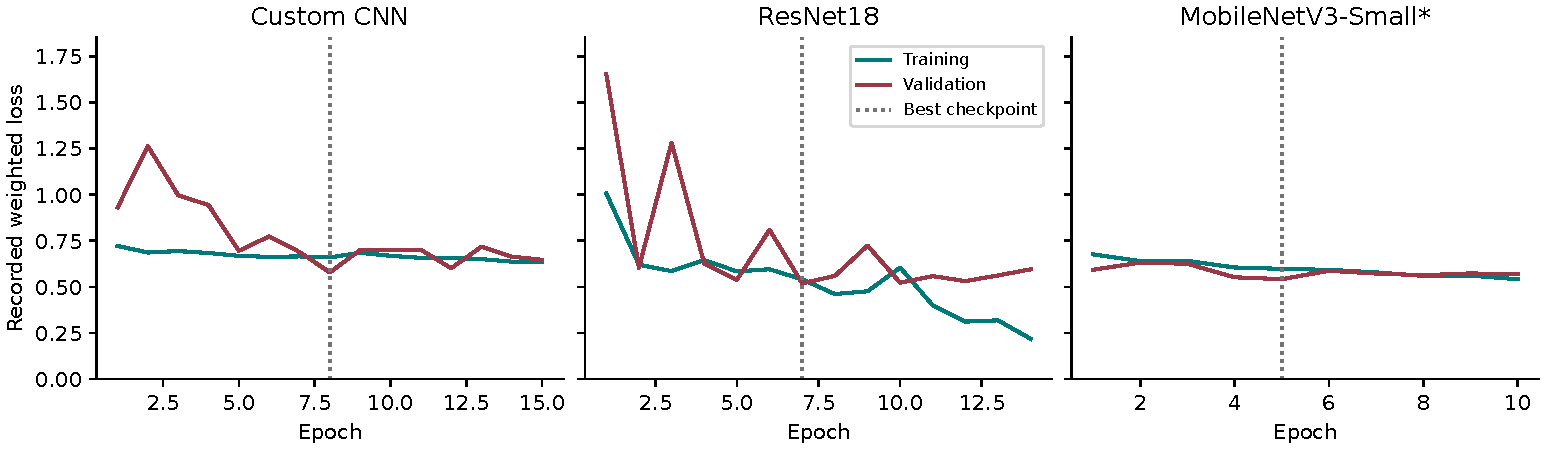
\includegraphics[width=\textwidth]{figures/training_histories.pdf}
\caption{Recorded training and validation weighted losses. Dotted lines identify retained checkpoints. MobileNet$^{*}$ is exploratory and trains only the classifier. Curves are within-run diagnostics; training configuration and trainable scope differ across models. No training was repeated to create this figure.}
\label{fig:history}
\end{figure}

Threshold selection substantially changed the original models' validation operating points (Table~\ref{tab:valthreshold}). Lowering their thresholds increased positive detection, accompanied by lower specificity. MobileNet's selected threshold was slightly above 0.5 and retained the same ten true positives while removing three false positives. The numerical distance from 0.5 is therefore less informative than the changed decision counts.

\begin{table}[htbp]
\centering\small
\caption{Validation operating points before and after selection. Both rows per model use the same saved validation scores; selected F1 was optimized on these data. Sensitivity and specificity refer to the positive and negative classes, respectively.}
\label{tab:valthreshold}
\begin{tabular}{llrrrr}\toprule
Model & Threshold & Precision & Sensitivity & Specificity & F1 \\\midrule
Custom CNN & 0.5 & 0.2000 & 0.1600 & 0.8462 & 0.1778 \\
 & Selected & 0.3721 & 0.6400 & 0.7404 & 0.4706 \\
ResNet18 & 0.5 & 0.5000 & 0.2400 & 0.9423 & 0.3243 \\
 & Selected & 0.3261 & 0.6000 & 0.7019 & 0.4225 \\
\mobile{}$^{*}$ & 0.5 & 0.5263 & 0.4000 & 0.9135 & 0.4545 \\
 & Selected & 0.6250 & 0.4000 & 0.9423 & 0.4878 \\\bottomrule
\end{tabular}
\par\source{Full validation threshold records, cross-checked against saved prediction CSVs.}
\end{table}

\subsection{Frozen-threshold test performance}
All test metrics in Table~\ref{tab:test} were checked against the original saved prediction CSVs and metric files. No new test inference was performed for this report. ResNet18 achieved the largest ROC-AUC (0.7473), AP (0.5220) and sensitivity (0.6400). MobileNet had the largest observed precision (0.5625), specificity (0.9327), F1 (0.4390) and accuracy (0.8217), at its own frozen threshold. Its balanced accuracy was 0.6463, compared with 0.6421 for ResNet18; this small observed difference is not evidence of statistical superiority.

\begin{table}[htbp]
\centering\small
\caption{Results on the common test partition: 129 images, including 25 positives. Threshold-dependent metrics use Table~\ref{tab:thresholds}. $^{*}$MobileNet was added post hoc; the expanded comparison is exploratory.}
\label{tab:test}
\begin{tabular}{lrrr}
\toprule
Metric & Custom CNN & ResNet18 & MobileNetV3-Small$^{*}$ \\
\midrule
ROC-AUC & 0.6123 & 0.7473 & 0.6562 \\
Average Precision & 0.4029 & 0.5220 & 0.4889 \\
Accuracy & 0.6124 & 0.6434 & 0.8217 \\
Balanced accuracy & 0.5317 & 0.6421 & 0.6463 \\
Precision & 0.2222 & 0.3019 & 0.5625 \\
Sensitivity & 0.4000 & 0.6400 & 0.3600 \\
Specificity & 0.6635 & 0.6442 & 0.9327 \\
F1-score & 0.2857 & 0.4103 & 0.4390 \\
\bottomrule
\end{tabular}

\par\source{\code{results/*_test/metrics.json} and \code{predictions.csv}; hashes and full-precision values retained in the evidence records.}
\end{table}

The count-level results explain the apparent disagreement between metrics (Figure~\ref{fig:cm}). The Custom CNN detected 10 positives and produced 35 false positives. ResNet18 detected 16 positives with 37 false positives. MobileNet detected nine positives with seven false positives, missing 16 of the 25 positive images. Its accuracy exceeded the always-homogeneous baseline by only two correctly classified images: 106 versus 104 out of 129.

\begin{figure}[htbp]
\centering
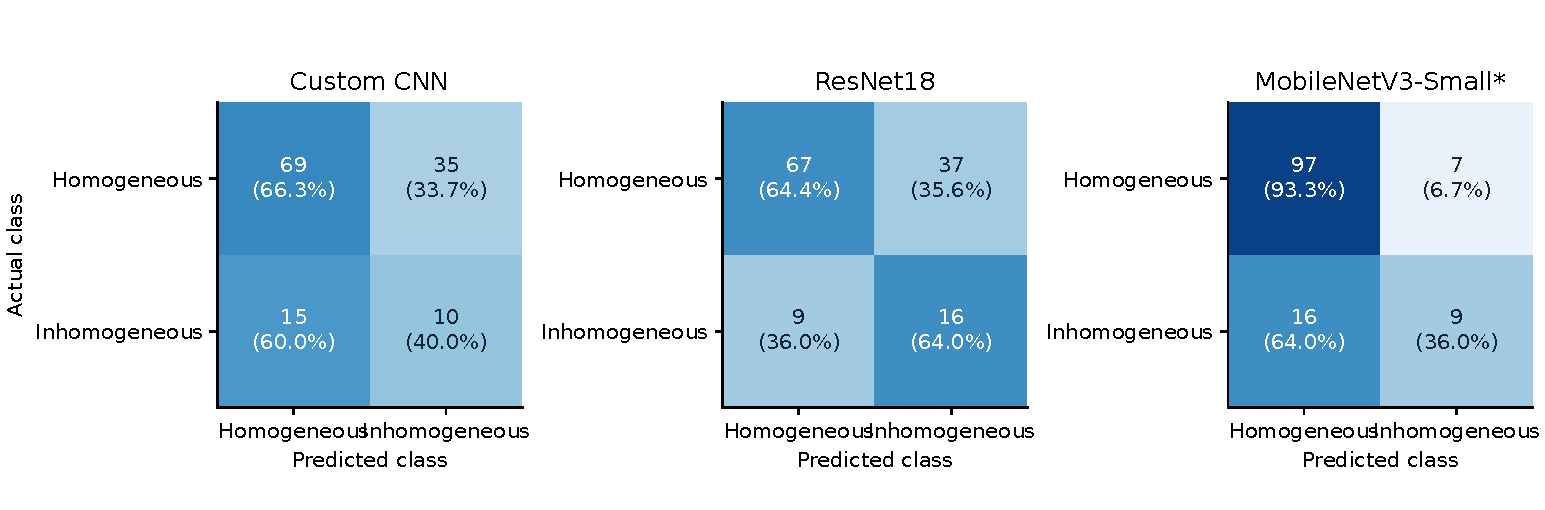
\includegraphics[width=\textwidth]{figures/confusion_matrices.pdf}
\caption{Frozen-threshold test confusion matrices. Cells give counts and percentages within the actual class; colour is normalized within each row. Rows are actual labels and columns are predictions. Class 0 is homogeneous; class 1 is inhomogeneous. All models use the same 104 homogeneous and 25 inhomogeneous images. $^{*}$Post-hoc exploratory model. Figure derived solely from saved prediction records.}
\label{fig:cm}
\end{figure}

\subsection{Validation versus test}
Table~\ref{tab:valtest} separates validation and test outcomes. Custom CNN F1 fell from 0.4706 to 0.2857, while ResNet18 F1 changed from 0.4225 to 0.4103. MobileNet F1 changed from 0.4878 to 0.4390. Ranking metrics do not move uniformly: ResNet18's test ROC-AUC and AP exceed its validation values, whereas the Custom CNN's ROC-AUC declines even as AP increases. These observations illustrate finite-sample variation and the different information captured by ranking summaries. They do not identify a particular source of distribution shift.

\begin{table}[htbp]
\centering\small
\caption{Partition-specific ranking and frozen-threshold metrics. Each validation/test partition contains 104 negatives and 25 positives. Validation F1 is the optimized selection result; test F1 is the subsequent observed result.}
\label{tab:valtest}
\begin{tabular}{llrrrrr}
\toprule
Model & Partition & AUC & AP & Sens. & Spec. & F1 \\
\midrule
Custom CNN & Validation & 0.7062 & 0.3195 & 0.6400 & 0.7404 & 0.4706 \\
Custom CNN & Test & 0.6123 & 0.4029 & 0.4000 & 0.6635 & 0.2857 \\
ResNet18 & Validation & 0.6919 & 0.3457 & 0.6000 & 0.7019 & 0.4225 \\
ResNet18 & Test & 0.7473 & 0.5220 & 0.6400 & 0.6442 & 0.4103 \\
MobileNetV3-Small & Validation & 0.6846 & 0.4631 & 0.4000 & 0.9423 & 0.4878 \\
MobileNetV3-Small & Test & 0.6562 & 0.4889 & 0.3600 & 0.9327 & 0.4390 \\
\bottomrule
\end{tabular}

\par\source{Saved validation/test probabilities and threshold configurations; \code{report/evidence.json}.}
\end{table}

One positive decision changes sensitivity by $1/25=0.04$. With only 25 positives in each partition, both the validation threshold optimum and the test sensitivity are sensitive to a few examples. No confidence intervals or paired significance tests were part of the frozen analysis. The report therefore treats the table as descriptive evidence and does not rank models by presumed statistical significance.

The original two validation metric JSONs contain one audit discrepancy: majority accuracy is recorded as 0.8093023, matching the full labelled dataset's $696/860$, rather than the partition's $104/129=0.8062016$. Model metrics and threshold sweeps reproduce correctly. The report uses the partition baseline and preserves both original files unchanged.

\subsection{Computational efficiency}
Table~\ref{tab:efficiency} reports the final trained-checkpoint benchmark. MobileNet's median 10.59 ms forward was approximately $62.17/10.59=5.9$ times faster than ResNet18 on this CPU. Its checkpoint was approximately 7.2 times smaller. The Custom CNN had the fewest parameters and smallest checkpoint, yet a larger measured median latency than MobileNet. Parameter count alone consequently did not predict runtime in this implementation.

\begin{table}[htbp]
\centering\small
\caption{Measured CPU model-forward latency and checkpoint size. Intel Core i7-7500U; float32; batch 1; $224\times224$ inputs; two intra-op threads, one inter-op thread; ten warm-ups and 50 timed forwards per model. MobileNetV3-Small is the post-hoc exploratory model.}
\label{tab:efficiency}
\begin{tabular}{lrrrrr}
\toprule
Model & Parameters & Checkpoint & Median & Mean & 95th pct. \\
 & & (MiB) & (ms) & (ms) & (ms) \\
\midrule
Custom CNN & 389,314 & 1.499 & 51.47 & 71.60 & 141.56 \\
ResNet18 & 11,177,538 & 42.713 & 62.17 & 71.48 & 106.72 \\
MobileNetV3-Small & 1,519,906 & 5.917 & 10.59 & 10.72 & 13.42 \\
\bottomrule
\end{tabular}

\par\source{\code{reports/model_efficiency.json}; all 50 raw measurements per model are retained.}
\end{table}

The Custom CNN mean (71.60 ms) exceeds its median (51.47 ms), and its 95th percentile reaches 141.56 ms. ResNet18 also varies across forwards. This variability prevents treating a median as a guaranteed service response time. The models were measured in one local benchmark sequence, without controlled thermal/load repeats across devices. Python 3.12.3, PyTorch 2.14.1+cpu and Torchvision 0.29.1+cpu identify that runtime. No end-to-end API latency, GPU comparison, power use or production throughput was measured.

\subsection{Explainability evidence}
Grad-CAM is implemented for all three architectures. The recorded application/container checks produce finite, nonconstant $224\times224$ maps on synthetic grayscale inputs and confirm unchanged predictions and parameter gradients after attribution. This verifies technical execution, including support for MobileNet's frozen features.

No archived original-ultrasound Grad-CAM images were found in the available results, artifacts or reports directories. Consequently, there is no qualitative anatomical finding to report and no medical overlay is presented. Synthetic heatmaps cannot demonstrate attention to testicular parenchyma, distinguish anatomical cues from annotations, or support clinical interpretation. The explainability contribution is an implemented inspection tool with bounded technical verification, rather than validated explanation quality.

\subsection{Deployment and reproducibility verification}
The previously completed development suite contains 150 passing tests, with no deselections and one Starlette TestClient deprecation warning. It covers data/split integrity, transforms, model interfaces, checkpoint restoration, thresholds, API behaviour, Grad-CAM and exploratory evaluation guards. This is the latest recorded application-suite result, not a new full-suite execution during report preparation. Four additional report-specific checks audit saved numeric evidence and generated tables without model execution.

Subsequent release preparation passed 18 tooling tests and one repository-hygiene test. It verified strict CPU loading of all three final checkpoints, preprocessing metadata and frozen thresholds without a model forward pass or dataset-image access (\code{release/verification.json}).

Earlier application checks reported 128 passes with one synthetic training test excluded. That test trains a fresh temporary CNN on random tensors for one epoch; it does not train a research checkpoint. The latest 150-test run included it and the analogous synthetic MobileNet test. The historical exclusion does not indicate a failed research experiment. Synthetic test training must also be distinguished from the separately authorized, now-frozen MobileNet research run.

For the original checkpoints, local CPU inference was compared with saved Colab probabilities on two validation samples per model. Maximum absolute differences were approximately $2.086\times10^{-7}$ for the Custom CNN and $1.788\times10^{-7}$ for ResNet18, with matching decisions. API and local command-line probabilities agreed in the sampled checks. MobileNet's validation threshold-candidate sample differed from its saved probability by approximately $1.192\times10^{-7}$ across local thread settings, with the same decision and exact API/CLI agreement.

Container checks used trained checkpoints with synthetic uploads for all three models and matched local probabilities exactly for those inputs. They verified health reporting, invalid-upload rejection, non-root execution, read-only filesystems/mounts and exclusion of artifact directories. A cached Docker build succeeded. An uncached PyTorch dependency download timed out, so a fresh network build was not demonstrated reliably. These checks establish consistency for sampled inputs and configured artifacts, not exhaustive numerical equivalence or a clean-network deployment guarantee.

\section{Discussion}
\subsection{What the comparison supports}
ResNet18 provides the strongest observed ranking of the positive class, alongside the highest sensitivity at its frozen operating point. This supports retaining it as a useful research comparator when detecting more positive images matters. It does not establish that transfer learning alone caused the improvement: network capacity, initialization and optimization all differ from the Custom CNN. A pretrained-versus-random ResNet ablation would be needed to isolate the initialization effect.

MobileNet offers a different operating point. It produces many fewer false positives and therefore greater precision and specificity, but detects fewer positives than ResNet18. Its higher accuracy is largely compatible with favouring the majority class. The nine true positives still improve on the zero detections of the majority baseline, yet the 16 missed positives prevent interpreting 82.17\% accuracy as broad success. Its AP is lower than ResNet18's despite higher frozen-threshold F1, showing why ranking quality and one decision point should be discussed separately.

The completed models therefore do not yield a universal winner. For example, relative to ResNet18, MobileNet has 30 fewer false positives but seven fewer true positives. Whether that exchange is desirable depends on a decision cost and workflow that this dataset does not provide. Selecting an architecture for patient care from these metrics would require an unmeasured clinical objective, not merely a different summary of the same table.

\subsection{Thresholds are part of the model's reported behaviour}
The validation analysis demonstrates why the default 0.5 decision rule was not adequate as an unexamined convention. The original models' lower selected thresholds detect more validation positives, although their specificity declines. MobileNet's small upward change removes some false positives without losing validation true positives. These are observed operating-point changes on fixed scores; threshold selection does not improve the representation or change ROC-AUC/AP.

Freezing and loading model-specific thresholds makes the deployed classifier correspond to the evaluated classifier. However, using a reproducible rule does not remove selection uncertainty. A maximum on 25 positive validation images may shift when only a few examples change. The validation F1 maximum is also selected from 129 candidates after checkpoint selection on the same validation data. Future work should estimate threshold stability within an appropriately grouped development design, reserving a genuinely untouched evaluation set for the final comparison.

Class-weighted training and validation thresholding act at different stages. Weighted loss alters optimization; the threshold turns a score into a label. Neither establishes probability calibration. A low numeric threshold should not be interpreted as a particular disease prevalence, risk tolerance or clinical alert policy.

\subsection{Efficiency and practical value}
MobileNet's observed latency and checkpoint size make it a credible candidate for further CPU-oriented research deployment. It reduces the resources required to demonstrate the full prediction interface, and its frozen-feature run was inexpensive on the available laptop. The experiment does not show that freezing features is the optimal training strategy or that a low-latency network has acceptable clinical performance.

The Custom CNN's larger latency despite fewer parameters is also informative. Its convolutional workload at high spatial resolutions, memory access and runtime kernels can matter alongside weight count; these are plausible explanations rather than measured bottleneck diagnoses. The benchmark establishes the observed runtime ordering under its stated conditions. Profiling and repeated hardware measurements would be needed to explain that ordering causally or generalize it to another device.

\subsection{Internal validity and the exploratory extension}
The fixed manifests and same test identities make numerical comparisons interpretable as predictions on the same images. Exact-duplicate and similarity checks address visible repetition, but cannot rule out correlated images from the same examination across partitions. Unknown grouping could make performance more optimistic than a new-patient evaluation. Conversely, the unexplained archive count difference prevents a confident claim to reproduce the precise official release.

MobileNet's protocol was declared before its training and its checkpoint/threshold were frozen before its own test evaluation. Those safeguards constrain within-experiment tuning. They do not undo the fact that the decision to add it followed observation of the first two test results. Reusing the same test partition makes the expanded comparison post hoc. It should guide future experiments, not serve as independent confirmation of architectural superiority. A new locked, patient-grouped external dataset would be required for that purpose.

\subsection{Limits of evidence and future work}
The principal constraints are the small labelled sample, imbalance, only 25 positive validation/test images, missing patient/examination and centre mappings, possible within-examination correlation, one training seed per configuration, threshold-selection uncertainty and absence of interval estimates. The original runs also lack some execution metadata. No centre-held-out validation, clinical validation, calibration assessment or prospective decision study was performed.

Future work should first resolve release provenance and obtain lawful patient/examination and per-image centre mappings. This would enable grouped splits, leakage checks and centre-held-out evaluation based on real acquisition metadata. A predeclared multi-seed comparison could then separate initialization, capacity and feature freezing through ablations; a classical feature baseline would broaden the evidence. Threshold selection and any calibration should remain inside development data, with grouped uncertainty analysis and a newly reserved evaluation partition.

For explanations, future work should archive attributed Grad-CAM examples selected under a declared sampling rule, include both correct and incorrect predictions, and test sensitivity to model/input changes. Expert comparison with anatomical regions could assess localization, but would still not establish causal reasoning or clinical usefulness. Deployment work should measure full request latency, concurrency and secure operating requirements on target hardware, and verify an uncached reproducible build when network access permits. These are proposed extensions, not experiments completed in this submission.

\subsection{Ethics, attribution and AI-assisted development}
This project uses a publicly released anonymized research dataset. The provider's 2026 manuscript describes full anonymization and reports ethics approval for the source data and annotations; those are provider-reported facts \citep{2026BMVC}. No separate institutional ethics approval, consent review or independent re-identification assessment for this student project is claimed. Predictions concern released image labels and must not be presented as diagnostic advice.

Dataset credit belongs to Morelli and colleagues and the TesticulUS contributors, with both the ICIAP 2025 and BMVC 2026 publications cited \citep{2025ICIAP,2026BMVC}. The source is \url{https://ditto.ing.unimore.it/testiculus/}. Original images and adapted ultrasound visualizations are governed by CC BY-NC-SA 4.0: \url{https://creativecommons.org/licenses/by-nc-sa/4.0/}. Noncommercial sharing and adaptation require attribution and the applicable ShareAlike terms \citep{cclicence}. Grad-CAM overlays, crops and other modified ultrasound images are adaptations; distribution must identify changes, retain attribution and licence links, and comply with ShareAlike. No dataset pixels are included in the report figures.

Independently developed software has its own applicable licensing and third-party terms. This repository currently declares no repository-wide software licence; the dataset licence does not supply one. Checkpoints and original ultrasound images remain outside Git under the project's artifact policy. A reviewer needs the separately supplied trained checkpoints and dataset access for full end-to-end execution.

AI assistance supported implementation, artifact verification, report drafting, evidence-linked tables/figures and document checks, as disclosed in \code{AI_USE.md}. Scientific responsibility, final factual review and the oral defence remain with the student. No new training, threshold change, held-out image inference or modification of experimental records was performed during report preparation.

\clearpage
\section{Conclusion}
This study delivers an auditable ultrasound image-classification pipeline and a reproducible research inference application. The original two-model comparison shows stronger observed test ranking and sensitivity for ResNet18 than the Custom CNN. The later exploratory MobileNet configuration offers lower measured CPU latency, smaller storage than ResNet18 and higher observed precision, specificity and F1 at its own frozen threshold, while missing most positive test images. These results support a performance--efficiency trade-off rather than a general claim of superiority.

The majority-class baseline demonstrates why accuracy alone would misrepresent the problem. Validation-selected thresholds expose and preserve a stated operating-point objective, and shared preprocessing/configuration loading connects that objective to API predictions. Grad-CAM and container checks extend reproducibility, but provide technical verification rather than scientific evidence of anatomical reasoning or clinical safety.

The defensible conclusion is limited to these configurations, this image-level split and the measured CPU runtime. Missing grouping metadata, uncertain release equivalence, one seed, few positive examples and the post-hoc third model constrain generalization. Patient-independent external evaluation, prospectively specified comparisons and clinical assessment remain necessary before any patient-care claim.

\FloatBarrier
\clearpage
\addcontentsline{toc}{section}{References}
\bibliographystyle{plainnat}
\bibliography{references}

\clearpage
\appendix
\section{Evidence map and reproducibility boundaries}
\label{app:evidence}
The report source, generated tables and figures are in \code{report/}. The machine-readable snapshot \code{report/evidence.json} retains full-precision reported values, histories, measured latency samples and a source SHA-256 map. It is a report derivative; original experimental records remain authoritative and unchanged. The accompanying \code{evidence_sources.md} details checks and unavailable information. Table~\ref{tab:evidencemap} maps the main claims to primary artifacts.

\begin{longtable}{>{\raggedright\arraybackslash}p{40mm}>{\raggedright\arraybackslash}p{110mm}}
\caption{Local evidence supporting the scientific report. Paths are relative to the repository root.}\label{tab:evidencemap}\\
\toprule Claim & Evidence \\\midrule\endfirsthead
\toprule Claim & Evidence \\\midrule\endhead
Dataset/split integrity & \code{data/splits/} and \code{reports/similarity_audit.md}; local dataset audit CSV. \\
Architectures and transforms & \code{src/models/architectures.py}; \code{src/data/transforms.py}; \code{src/data/dataset.py}. \\
Training and histories & \code{src/training.py}; original checkpoint metadata in \code{reports/artifact_verification.json}; \code{training_runs/*/history.csv}; MobileNet freeze/training summary. \\
Threshold procedure & \code{src/threshold_selection.py}; \code{src/threshold_config.py}; original and separate MobileNet threshold JSONs. \\
Frozen test results & \code{results/*_test/metrics.json} and \code{predictions.csv}; \code{reports/mobilenet_exploratory_results.json}. \\
Exploratory ordering & \code{reports/mobilenet_exploratory_protocol.json}; \code{reports/mobilenet_v3_small_freeze.json}; local evaluation receipt. \\
Latency measurements & \code{reports/model_efficiency.json}; \code{src/cpu_benchmark.py}. \\
Grad-CAM/API & \code{src/gradcam.py}; \code{src/inference.py}; \code{src/api.py}; saved artifact/application verification JSONs. \\
Docker & \code{Dockerfile}; \code{.dockerignore}; saved original/MobileNet container verification reports. \\
Tests and disclosure & \code{tests/}; \code{docs/mobilenet_experiment.md}; \code{AI_USE.md}; report-only tests. \\\bottomrule
\end{longtable}

The original Custom CNN and ResNet18 checkpoints and artifacts were supplied from Google Drive under \code{MyDrive/Capstone/}, mirrored in \code{training_runs/} and \code{results/}; the exploratory MobileNet checkpoint was produced locally. This describes historical provenance. Source code is maintained at \url{https://github.com/mweneh/testiculus-ultrasound-classification}; the chosen checkpoint distribution channel is separate GitHub Releases. Examiners should use the matching supplied source checkout pending an authorized push of the submission commits. The prepared tag \code{models-v1.0.0} was not found by a GitHub release query on 19 November 2026. Public checkpoint download is therefore not claimed. Owner review of redistribution terms and authorized publication remain outstanding; \code{release/README.md} records that step.

\begin{samepage}
The prepared local package is in \path{artifacts/releases/models-v1.0.0/}. It contains both complete threshold JSONs and these checkpoints:
\begin{itemize}
\item Custom CNN: \code{testiculus-custom-cnn-v1.pth}.
\item ResNet18: \code{testiculus-resnet18-v1.pth}.
\item Exploratory MobileNet: \code{testiculus-mobilenet-v3-small-v1.pth}.
\end{itemize}
\end{samepage}
Examiners can use the README's Python 3.12 serving environment (verified host: 3.12.3), verify \code{SHA256SUMS} from the package directory and use the following commands from the repository root:
\begin{verbatim}
PKG=artifacts/releases/models-v1.0.0
python -m src.release_assets verify --package "$PKG"
python -m src.inference --device cpu \
  --checkpoint "$PKG/testiculus-resnet18-v1.pth" \
  --threshold-config "$PKG/validation_thresholds.json" \
  --image /path/to/research-image.png
\end{verbatim}
The verifier checks assets against the trusted source manifest before strict CPU loading. Custom CNN uses the same threshold JSON; MobileNet uses \path{mobilenet_v3_small_thresholds.json}. After publication, the optional downloader installs under \path{artifacts/checkpoints/models-v1.0.0/}; the same commands accept that directory. The README also gives a read-only Docker mount for these flat asset names. Checkpoint binaries remain outside ordinary Git commits. Hashes establish consistency with supplied bytes, not independently authenticated Colab provenance.

The owner-confirmed alternative channel is Strathmore University Virtual Campus, DSA 8401, \emph{Capstone Project (23 Nov)} assignment submission, supplying the matching source checkout and complete checkpoint package. Upload and examiner-access verification are pending. GitHub Releases remains preferred, with the repository URL submitted through Virtual Campus. The assignment label does not change this report's recorded submission deadline.

ResNet's current initialization source is Torchvision's \code{resnet18-f37072fd.pth}, and MobileNet's recorded source is \code{mobilenet_v3_small-047dcff4.pth}, both under \url{https://download.pytorch.org/models/}. Inference restores complete trained states with pretrained downloading disabled. The original ResNet initialization file itself was not independently fingerprinted in the retained Colab metadata.

The report follows the supplied DSA 8401 instructions; no institutional template or approved proposal was found. The ICIAP 2025 reference now uses Springer's final record: pages 26--39, DOI \code{10.1007/978-3-032-10192-1_3}, published 2 January 2026. Its conference year remains 2025; the bibliography uses the 2026 publication year. The original provider entries remain unchanged in \code{data/references.bib} and the prepared release's BibTeX file; release notes identify the final published record. The BMVC citation and dataset attribution are retained.

\clearpage
\section{Rebuilding this document without rerunning experiments}
From the repository root, the following checks read saved records and never open ultrasound images or execute models:
\begin{verbatim}
OMP_NUM_THREADS=1 .venv/bin/python -m unittest \
  discover -s report -p 'test_*.py' -v
MPLCONFIGDIR=/tmp/capstone-matplotlib .venv/bin/python \
  report/build_evidence.py --verify-local --check
\end{verbatim}
The first and second commands require local numeric CSV artifacts. On a checkout without those files, figures and tables can be rebuilt from the committed snapshot using \code{report/build_evidence.py} without \code{--verify-local}. The PDF build itself needs no dataset, checkpoints or Python packages:
\begin{verbatim}
cd report
pdflatex -interaction=nonstopmode -halt-on-error capstone_report.tex
bibtex capstone_report
pdflatex -interaction=nonstopmode -halt-on-error capstone_report.tex
pdflatex -interaction=nonstopmode -halt-on-error capstone_report.tex
\end{verbatim}

The full application suite's recorded 150-pass result is distinct from the report's four additional checks. The full suite is not rerun here because report preparation does not require synthetic model optimization. Inference and Docker execution commands are maintained in the repository README and \code{docs/mobilenet_experiment.md}; they are not duplicated as experimental methods. Existing training/test commands document the frozen work and must not be rerun to revise these results.

Remaining author checks are approval of the final prose and scope statement, institutional submission details, redistribution review and authorized release publication, and confirmation of examiner access to the separately supplied artifacts. These checks do not require altering any scientific result.
\end{document}
